\documentclass{article}
\usepackage{amsmath,amssymb}
\usepackage{tikz}
\usetikzlibrary{arrows.meta,positioning,calc,shapes.geometric}
\pagestyle{empty}
\begin{document}
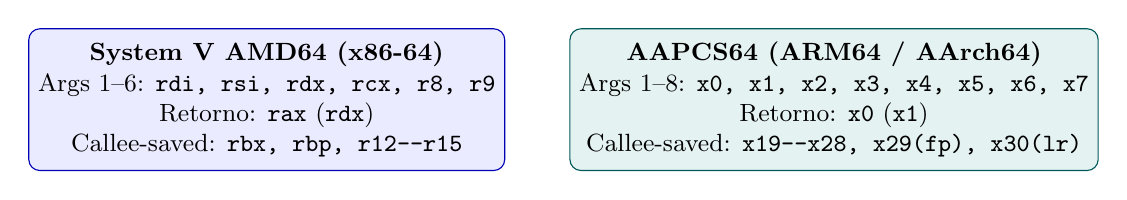
\begin{tikzpicture}
\tikzset{node distance=1.4cm, >=stealth, thick, font=\small}
\node[draw=blue!70!black, fill=blue!8, rounded corners, minimum width=5.6cm, minimum height=1.8cm, align=center] (x86) {\textbf{System V AMD64 (x86-64)}\\Args 1--6: \texttt{rdi, rsi, rdx, rcx, r8, r9}\\Retorno: \texttt{rax} (\texttt{rdx})\\Callee-saved: \texttt{rbx, rbp, r12--r15}};
\node[draw=teal!70!black, fill=teal!10, rounded corners, minimum width=5.6cm, minimum height=1.8cm, align=center, right=0.8cm of x86] (arm) {\textbf{AAPCS64 (ARM64 / AArch64)}\\Args 1--8: \texttt{x0, x1, x2, x3, x4, x5, x6, x7}\\Retorno: \texttt{x0} (\texttt{x1})\\Callee-saved: \texttt{x19--x28, x29(fp), x30(lr)}};
\end{tikzpicture}
\end{document}
